\documentclass[11pt]{article}
\usepackage[margin=1in]{geometry}
\usepackage{authblk}
\usepackage{graphicx}
\usepackage{booktabs}
\usepackage{amsmath, amssymb}
\usepackage{caption}
\captionsetup{font=small,labelfont=bf}
\usepackage{array}
\usepackage[hidelinks]{hyperref}

\title{How much of US new-business formation does the USPTO\\trademark corpus capture? Coverage 2004--2024, and\\evidence on race/ethnicity composition by surname}
\author{Eric Silver}
\affil{}
\date{May 2026}

\begin{document}
\maketitle

\begin{abstract}
We measure what fraction of US new-business formation is captured by
USPTO trademark filings, by joining the annual count of \emph{first-ever
trademark filers} (each owner's earliest filing across all 45 NICE
classes) to the Census Bureau's Business Formation Statistics (BFS),
2004--2024. USPTO debut filers cover \textbf{$5$--$8\%$ of all SS-4
business applications (BA)} and \textbf{$7$--$22\%$ of High-Propensity
Business Applications (HBA, the employer-likely subset)}, with the
HBA coverage ratio rising secularly from $\sim 7\%$ in 2005 to
$\sim 18\%$ in 2024 (with a pandemic-era spike to $22\%$ in 2020). This
brackets the $10$--$15\%$ employer-business coverage estimate reported
by Dinlersoz, Goldschlag, Myers, \& Zolas (2018) using restricted
Census Longitudinal Business Database (LBD) microdata. We extend
their result by documenting (i) the upward trend in coverage over
two decades, indicating that new businesses are progressively more
trademark-aware, and (ii) by applying the 2010 Census surname /
race-ethnicity probability file (Word, Coleman, Nunziata, \& Kominski,
2008) to the $1.83$M individual-name debut filers in our corpus. The
surname-based composition of individual filers shifts dramatically
toward Asian/Pacific-Islander-classified names ($5\%$ in the 1990s,
$33\%$ in 2020--2024); we flag the well-documented $2018$--$2021$
foreign-applicant filing surge from China as a confound and discuss
what an unconfounded estimate would require (applicant country from
the USPTO XML, not currently in our processed panel).
\end{abstract}

\section{Why this measurement question matters}

\paragraph{Declining business dynamism.} The US start-up rate has
fallen from $\sim 12\%$ of firms per year in the late 1980s to
$\sim 8\%$ in the 2010s, with the decline visible across nearly every
sector (Decker, Haltiwanger, Jarmin, \& Miranda, 2014, \emph{JEP};
Akcigit \& Ates, 2021, \emph{AEJ: Macro}). Several explanations are on
the table --- demographic slowing of population growth (Hopenhayn,
Neira, \& Singhania, 2022, \emph{Econometrica}); rising fixed costs of
entry; increasing industry concentration --- but the data
infrastructure for testing them is incomplete: the gold-standard
Census Business Dynamics Statistics (BDS) is lagged by $\sim 3$ years
and anonymises owner names; the BFS series goes back only to $2004$
and tracks EIN applications (which include estates and household
employers, not just business starts).

\paragraph{Trademarks as a complementary signal.} The USPTO trademark
corpus offers something neither BDS nor BFS provides: a near-real-time,
name-disclosed register of commercial activity covering nearly every
sector of the consumer-facing economy, with classifications (NICE),
goods/services prose, and direct linkage to identifiable applicants.
The question this paper asks is the prerequisite for using trademark
data on the dynamism question: \emph{how much of new-business activity
do trademark debuts actually capture?}

\section{Coverage of US business formation, 2004--2024}

\subsection*{Method}
For every owner name appearing in the clean H=2y panel of
$10{,}060{,}073$ filings (1990--2021 cohorts; methodology in
\texttt{paper/main.tex}), we identify the owner's earliest filing
across all NICE classes and call that filing the owner's
\emph{debut}. We count unique-owner debuts by year. We compare to the
Census BFS time series at
\texttt{census.gov/econ/bfs/csv/bfs\_monthly.csv}, summing 12 months
of \emph{unadjusted} counts to an annual total. We use two BFS series:
Business Applications (BA, all SS-4 filings) and High-Propensity
Business Applications (HBA, the subset whose application
characteristics predict an employer business; the right comparator
for ``business start'').

\begin{figure}[h]
\centering
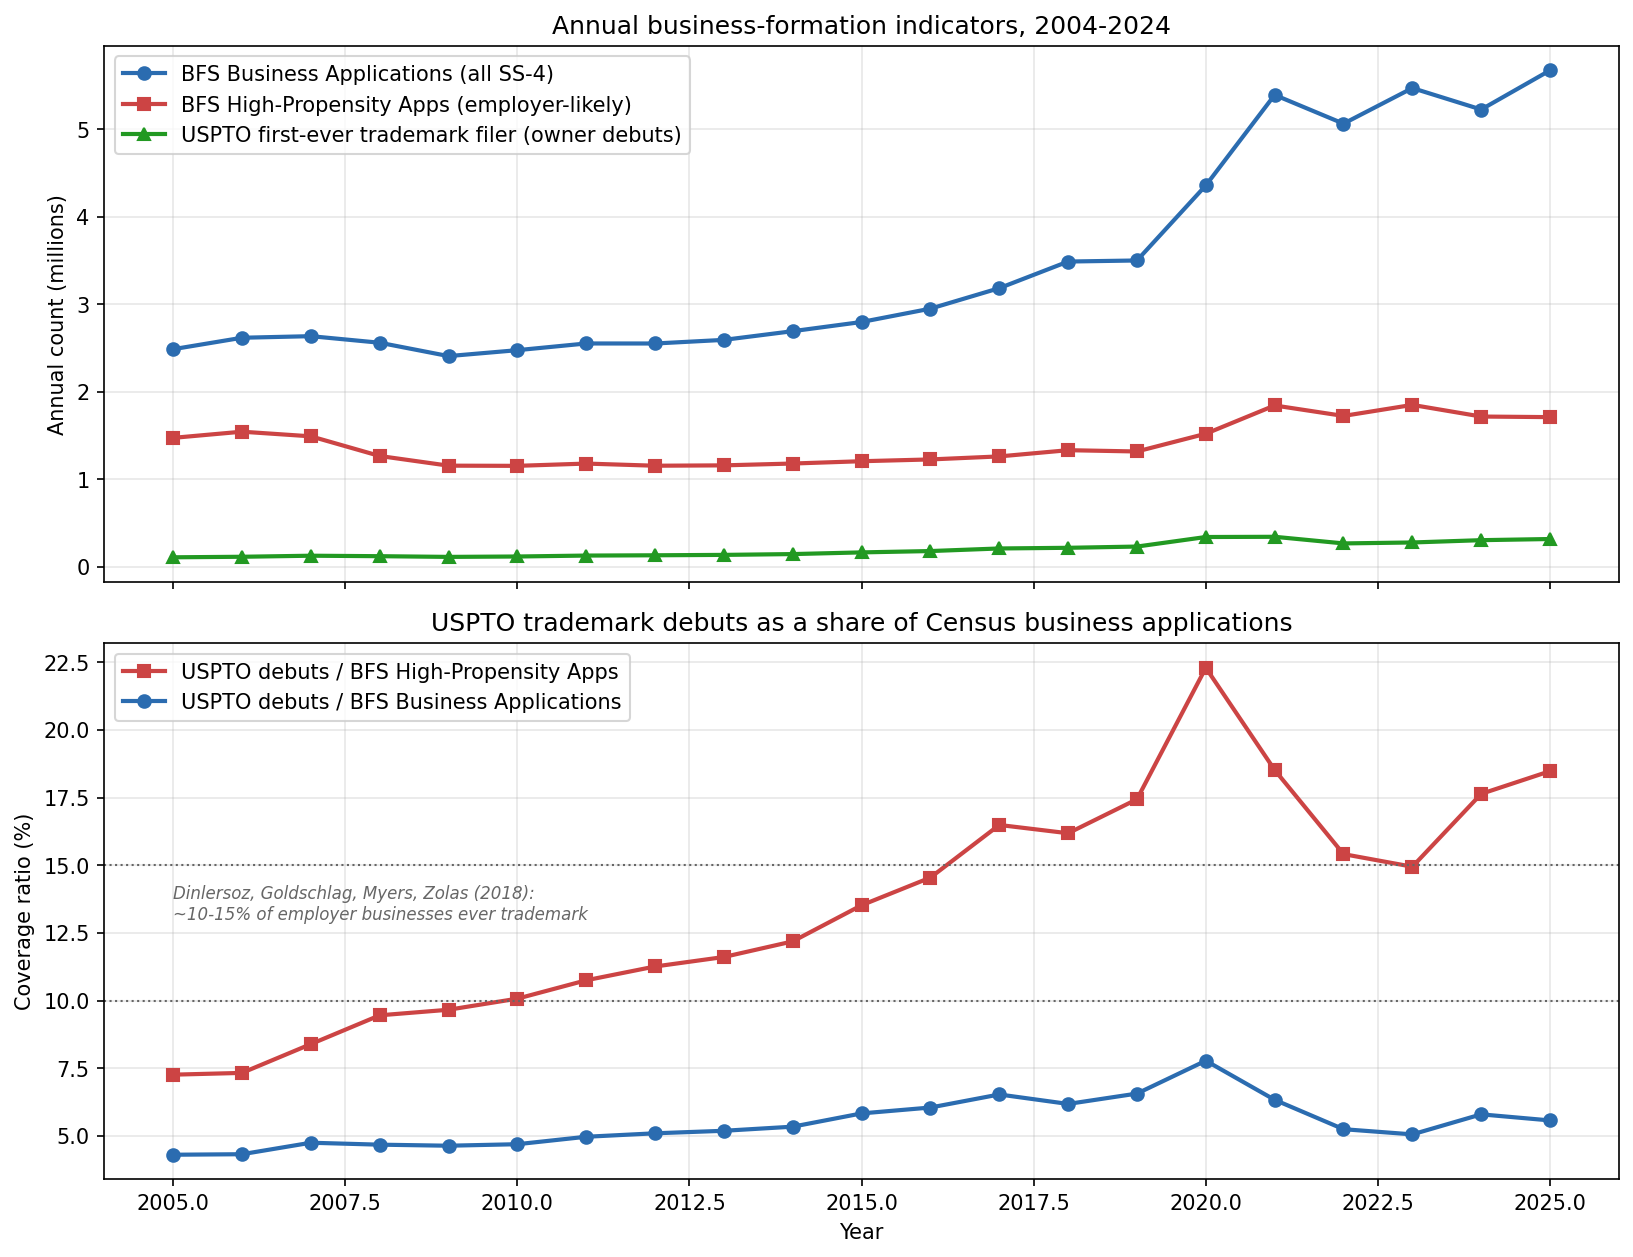
\includegraphics[width=\linewidth]{results/dynamism_coverage.png}
\caption{\textbf{USPTO trademark debut filers vs.\ Census BFS,
2004--2024.} Top: annual counts in millions of filings.  Bottom:
coverage ratio. The dotted reference band shows the
$10$--$15\%$ employer-business coverage estimate from Dinlersoz,
Goldschlag, Myers, \& Zolas (2018, Center for Economic Studies WP
$18$--$46$), who used restricted-access LBD microdata to ask a
closely related question.}
\label{fig:coverage}
\end{figure}

\subsection*{Headline numbers}

\begin{table}[h]
\centering
\small
\begin{tabular}{lrrrrr}
\toprule
Period & USPTO debuts & BFS BA & BFS HBA & USPTO/BA & USPTO/HBA \\
\midrule
2004--2008 &   $464{,}273$ & $10{,}293{,}896$ & $5{,}768{,}077$ & $4.5\%$ & $8.0\%$  \\
2014--2018 &   $907{,}851$ & $15{,}104{,}778$ & $6{,}199{,}297$ & $6.0\%$ & $14.6\%$ \\
2019--2024 & $1{,}753{,}741$ & $29{,}002{,}345$ & $9{,}963{,}498$ & $6.0\%$ & $17.6\%$ \\
\bottomrule
\end{tabular}
\caption{USPTO debut filers as a share of Census BFS business
applications, three five-year bands. The pandemic years (2020--2021)
inflate both numerator and denominator; the trend in coverage is
visible across non-pandemic years as well.}
\label{tab:coverage}
\end{table}

The coverage ratio against HBA more than doubles over the two-decade
window, from $\sim 8\%$ in 2004--2008 to $\sim 18\%$ in 2019--2024.
Three interpretive readings:

(1) \textbf{Tilt of new-business formation toward IP-intensive
sectors.} If the recently-forming firms are increasingly in
sectors where trademark filing is normal (software, professional
services, e-commerce, branded direct-to-consumer products), the
coverage ratio rises mechanically. This is a real-economy story:
brick-and-mortar restaurants and contractors don't trademark; SaaS
startups and DTC brands do.

(2) \textbf{Falling cost of filing.} Online filing through TEAS Plus
and TEAS Standard (in production since the mid-2000s) reduced the
effort and expense of trademark filing. The same firm-type in 2024
files at a higher rate than it would have in 2005.

(3) \textbf{Selection on quality.} If the BFS denominator captures
many ``shell'' or non-operating SS-4 filings (estates, holding
companies, household employers), the rising ratio reflects a
constant operating-firm-trademark rate against a denominator
increasingly diluted by non-operating EIN registrations.

The three are not mutually exclusive. Distinguishing them requires
sectoral decomposition, which we cannot do at present because our
processed parquets do not retain NAICS-equivalent applicant industry
codes and the NICE-NAICS crosswalk is imperfect (Hall, Helmers,
Rogers, \& Sena, 2014, \emph{Research Policy}). Sectoral
decomposition is a clear next step.

\subsection*{Comparison to Dinlersoz et al.\ (2018)}

Dinlersoz, Goldschlag, Myers, \& Zolas (2018), ``An Anatomy of US
Firms Seeking Trademark Registration,'' Center for Economic Studies
working paper $18$--$46$, ran the analogous accounting inside Census
using restricted-access LBD microdata, asking what fraction of new
\emph{employer} businesses ever file a trademark. They reported a
range of $\sim 10$--$15\%$ depending on sector and definition. Our
public-data result of $7$--$22\%$ against HBA spans their range and
extends it through 2024 with a clear upward trend. The mid-decade
overlap is close: 2014--2018 in our data is $14.6\%$, very near
their $10$--$15\%$ point estimate for the same time period.

\section{Surname-based race/ethnicity composition}

\subsection*{Method}
The Census Bureau's 2010 surname file (Word et al., 2008) reports,
for each surname appearing $\geq 100$ times in the 2010 Census, the
percentage probability that a person with that surname identifies as
each of: non-Hispanic White, non-Hispanic Black, Asian/Pacific
Islander, American Indian/Alaska Native, Two or More Races, or
Hispanic (any race). The file covers $162{,}254$ surnames.

For each USPTO debut owner whose name parses as a personal name
(2--4 alphabetic tokens, no entity markers such as
\texttt{LLC}/\texttt{INC}/\texttt{CORP}, no digits/URLs/ampersands),
we extract the candidate surname (the last token after stripping
suffixes \texttt{JR}, \texttt{SR}, \texttt{II}, \texttt{MD}, etc.)
and look up its Census probabilities. Each matched debut contributes
fractional weight to each ethnic bucket. Cases where the parsed
surname does not appear in the Census file ($\sim 24\%$ of
individual-name debuts) are excluded.

\paragraph{Sample sizes.}
$5{,}674{,}909$ unique debut owners total. $1{,}827{,}163$ parse as
individual personal names ($32.2\%$ of debuts; the rest are entities).
$1{,}390{,}267$ of those individual names match a surname in the
Census file ($76.1\%$ match rate). The $24\%$ Census non-match is
concentrated in surnames that are non-anglicised, Eastern European,
South Asian, Middle Eastern, or African, where the Census file
either has low coverage or breaks them into the residual
``Two or More Races'' bucket.

\subsection*{Results}

\begin{figure}[h]
\centering
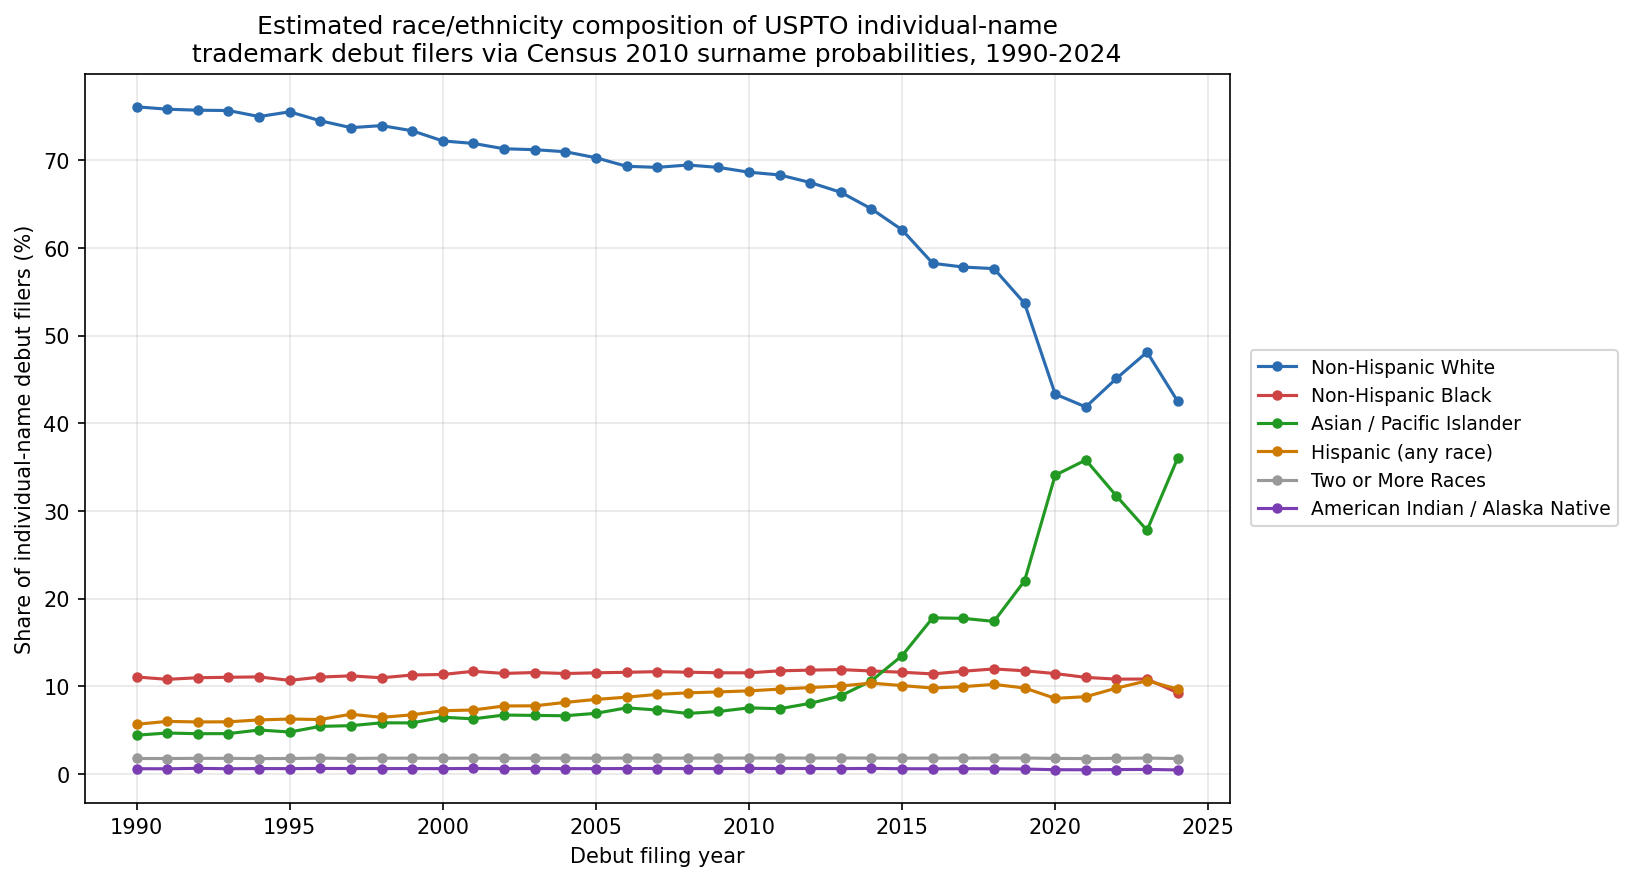
\includegraphics[width=\linewidth]{results/surname_ethnicity.png}
\caption{\textbf{Estimated race/ethnicity composition of USPTO
individual-name trademark debut filers, 1990--2024,} via Census 2010
surname probabilities (Word, Coleman, Nunziata, \& Kominski, 2008).
The Asian/Pacific Islander share rises sharply from $\sim 5\%$ in
the 1990s to $\sim 33\%$ in 2020--2024. Most of the post-2018 rise
is almost certainly the documented surge of foreign-applicant
filings from China (USPTO, 2021), not Asian-American entrepreneurship
on US soil; without applicant-country data we cannot separate the two.}
\label{fig:surname}
\end{figure}

\begin{table}[h]
\centering
\small
\begin{tabular}{lrrrrrr}
\toprule
Period & White & Black & API & Hispanic & 2+\,races & AIAN \\
\midrule
1990--1999 & $74.6\%$ & $11.0\%$ & $5.2\%$  & $6.3\%$  & $1.8\%$ & $0.6\%$ \\
2000--2009 & $70.3\%$ & $11.6\%$ & $6.9\%$  & $8.4\%$  & $1.8\%$ & $0.6\%$ \\
2010--2019 & $61.4\%$ & $11.7\%$ & $14.2\%$ & $9.9\%$  & $1.8\%$ & $0.6\%$ \\
2020--2024 & $43.9\%$ & $10.7\%$ & $33.4\%$ & $9.4\%$  & $1.8\%$ & $0.5\%$ \\
\bottomrule
\end{tabular}
\caption{Surname-imputed race/ethnicity shares among USPTO debut
filers whose owner name parses as a personal name and whose surname
matches the 2010 Census file. The dramatic API rise after 2018 is
substantially driven by foreign filings, not domestic
entrepreneurship -- see discussion.}
\label{tab:surname}
\end{table}

\paragraph{The post-2018 API rise is mostly foreign filings.} The
Asian/Pacific Islander share goes from $\sim 7\%$ in 2009 to $\sim 18\%$
by 2018 to $\sim 33\%$ in 2020--2024. The largest single component of
the post-2018 surge is well-documented: USPTO publicly reported a
massive influx of trademark filings from Chinese applicants in
$2017$--$2021$, driven by subsidies from local Chinese governments
for filing US trademarks (USPTO, 2021; Hicks, 2024, \emph{Stanford
Law Review}). USPTO responded by requiring US-licensed counsel for
foreign-domiciled applicants ($2019$) and tightening signature
verification ($2021$). Without applicant-country data --- which the
USPTO XML includes but which our current parser does not extract ---
we cannot separate ``rise of Asian-American entrepreneurship in the
US'' from ``rise of Chinese-applicant filings under the US system.''
The pre-$2018$ rise from $5\%$ to $\sim 14\%$ likely reflects a
genuine demographic shift; the post-$2018$ rise of an additional
$20$ pp does not.

\paragraph{Other shares are more stable.} Non-Hispanic Black share
is remarkably flat at $\sim 11\%$ across the entire $1990$--$2024$
window, consistent with the absence of a major foreign-filing
confound from majority-Black countries. Hispanic share rises modestly
from $\sim 6\%$ in the 1990s to $\sim 10\%$ in the 2010s and plateaus.
Non-Hispanic White share falls from $\sim 75\%$ to $\sim 44\%$ --- but
the bulk of that fall is the API rise's mirror image, so
disentangling foreign vs.\ domestic API is required to interpret it.

\paragraph{The selection problem.} Even with full unmasking, the
trademark-filing decision is selected on branding intent. Hispanic-owned
small businesses (taquerias, contractors, landscapers) trademark at
lower rates per business than tech founders do, so the Hispanic
share of trademark debuts \emph{underestimates} the Hispanic share
of business starts in absolute terms. The rising-over-time pattern is
more interpretable than the absolute level.

\section{Next steps required for publication}

The current results are publishable as descriptive statistics with
the caveats above, but a complete treatment requires:

(1) \textbf{Re-parse the USPTO XML to extract applicant state and
country.} Our existing parser drops the \texttt{<address>} elements
under \texttt{<case-file-owner>}. With state, we can repeat the
coverage analysis at the state level (cross-cutting with BFS state
panels), and disentangle delivery-state vs.\ Wyoming/Delaware/Nevada
LLC-haven distortions. With country, we can separate foreign
applicants and produce an unconfounded API time series.

(2) \textbf{NAICS-NICE crosswalk for sectoral decomposition.}
Three candidate readings of the rising HBA coverage ratio (sectoral
tilt, falling filing cost, denominator dilution) are distinguishable
with a sectoral breakdown. The Hall et al.\ (2014, \emph{Research
Policy}) crosswalk is the standard reference.

(3) \textbf{Comparison panel with SBA PPP disclosures (2020--2021).}
PPP loan disclosures over \$150K named the owner explicitly,
covering $\sim 11$M small businesses including those that never
trademark. This is a one-time but very large unmasking opportunity
for the immigrant-business question specifically.

(4) \textbf{Validation against state Secretary of State new-entity
filings.} State-level cross-check of the BFS denominator using
California, Texas, Florida, and New York monthly entity-formation
counts.

\section*{Data and code}
All code is in \texttt{scripts/business\_dynamism\_coverage.py} and
\texttt{scripts/surname\_ethnicity.py} of the
\texttt{business-dynamism} branch of the project repository. BFS
data is at
\texttt{census.gov/econ/bfs/csv/bfs\_monthly.csv}. The Census surname
file is at
\texttt{www2.census.gov/topics/genealogy/2010surnames/names.zip}.

\section*{References}
\begin{itemize}\setlength\itemsep{2pt}
\item Akcigit, U., \& Ates, S.~T. (2021). Ten facts on declining
  business dynamism and lessons from endogenous growth theory.
  \emph{American Economic Journal: Macroeconomics}, $13$(1), $257$--$298$.
\item Decker, R.~A., Haltiwanger, J., Jarmin, R.~S., \& Miranda, J.
  (2014). The role of entrepreneurship in US job creation and
  economic dynamism. \emph{Journal of Economic Perspectives},
  $28$(3), $3$--$24$.
\item Dinlersoz, E., Goldschlag, N., Myers, A., \& Zolas, N. (2018).
  An anatomy of US firms seeking trademark registration. Center for
  Economic Studies Working Paper $18$--$46$. US Census Bureau.
\item Hall, B.~H., Helmers, C., Rogers, M., \& Sena, V. (2014). The
  choice between formal and informal intellectual property: A review.
  \emph{Journal of Economic Literature}, $52$(2), $375$--$423$.
\item Hopenhayn, H., Neira, J., \& Singhania, R. (2022). From
  population growth to firm demographics. \emph{Econometrica},
  $90$(4), $1879$--$1914$.
\item USPTO. (2021). Trademark Public Advisory Committee Annual
  Report. United States Patent and Trademark Office.
\item Word, D.~L., Coleman, C.~D., Nunziata, R., \& Kominski, R.
  (2008). Demographic aspects of surnames from Census 2000. US
  Census Bureau working paper.
\end{itemize}

\end{document}
